%%---------------------------------------------------------------------------%%
%% budgets.tex
%%---------------------------------------------------------------------------%%

\addcontentsline{toc}{section}{\protect\numberline{}Budgets}
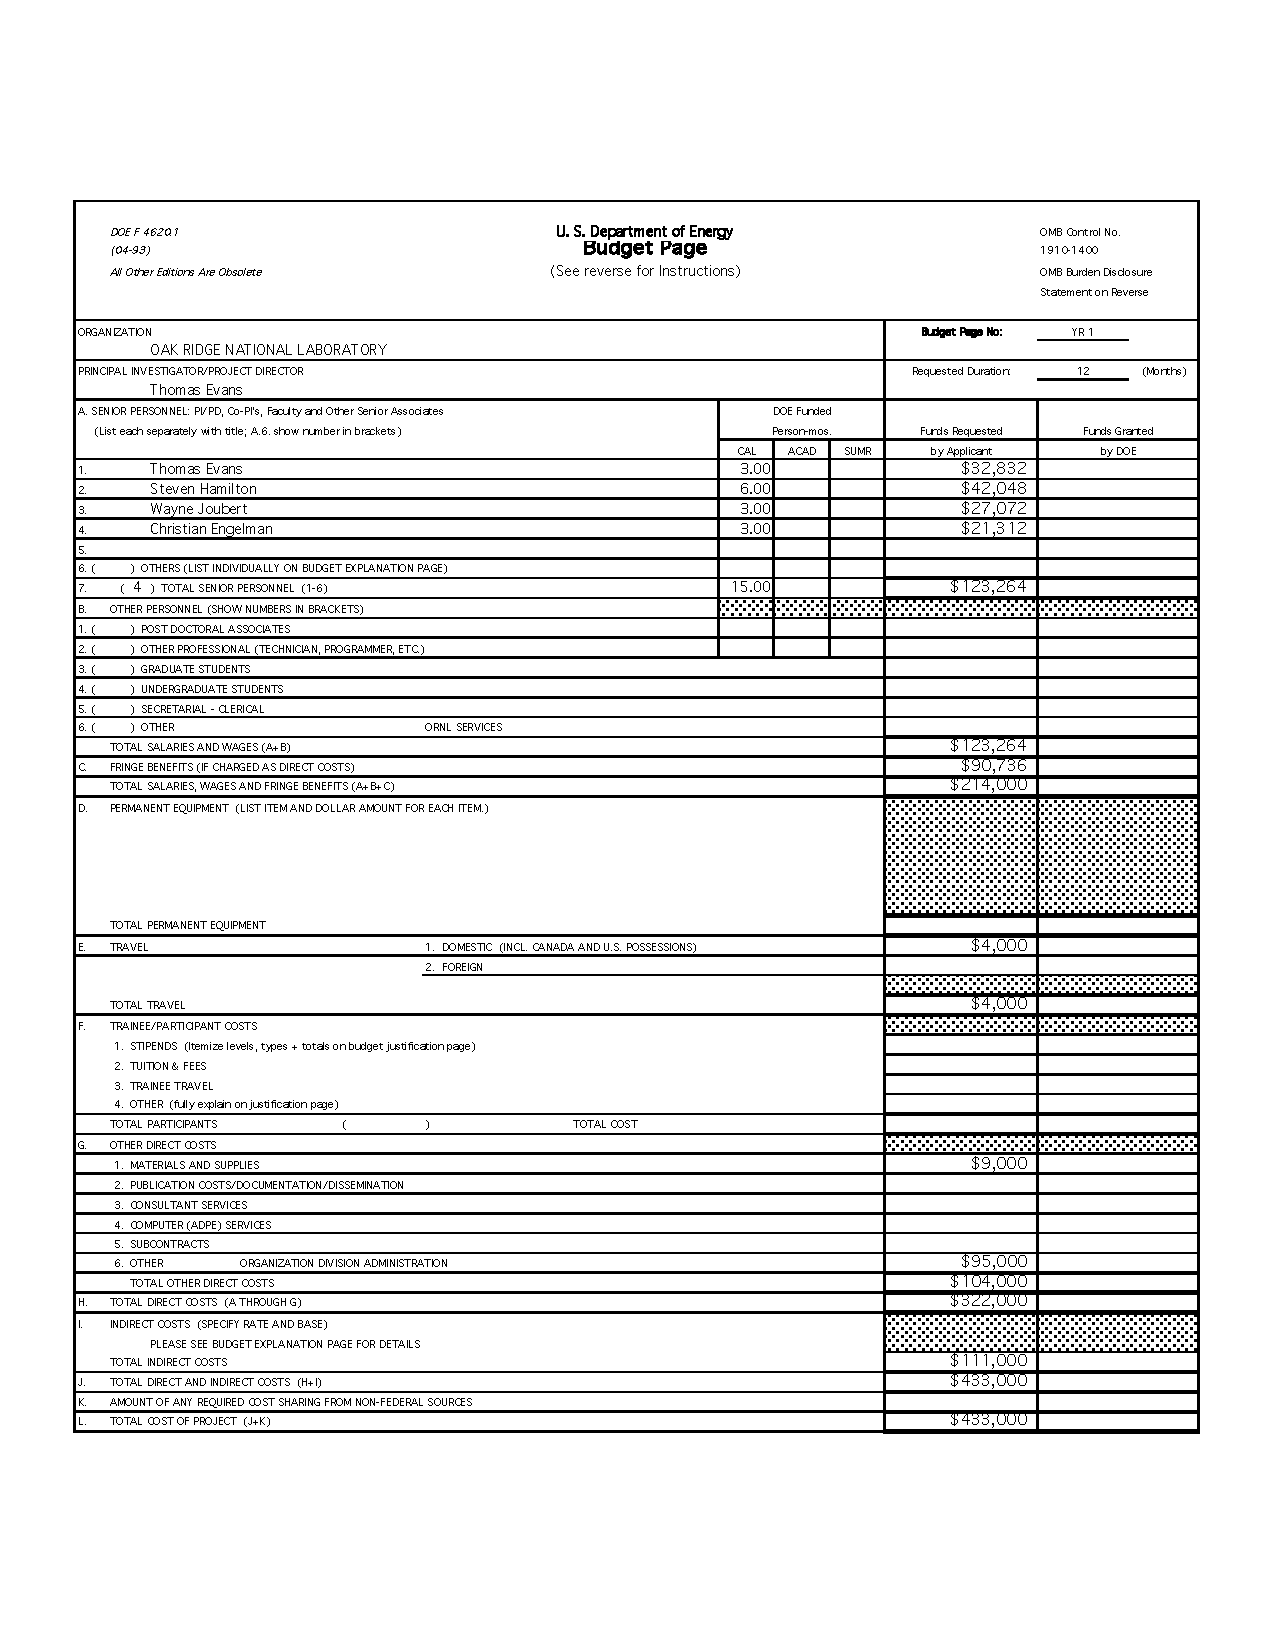
\includepdf[pages=-,pagecommand={\section*{Budgets}\subsection*{ORNL Budget}
  \thispagestyle{fancy}}, noautoscale=true,scale=0.9] {supp/doe_4620_1}
\addcontentsline{toc}{subsection}{\protect\numberline{}ORNL Budget}
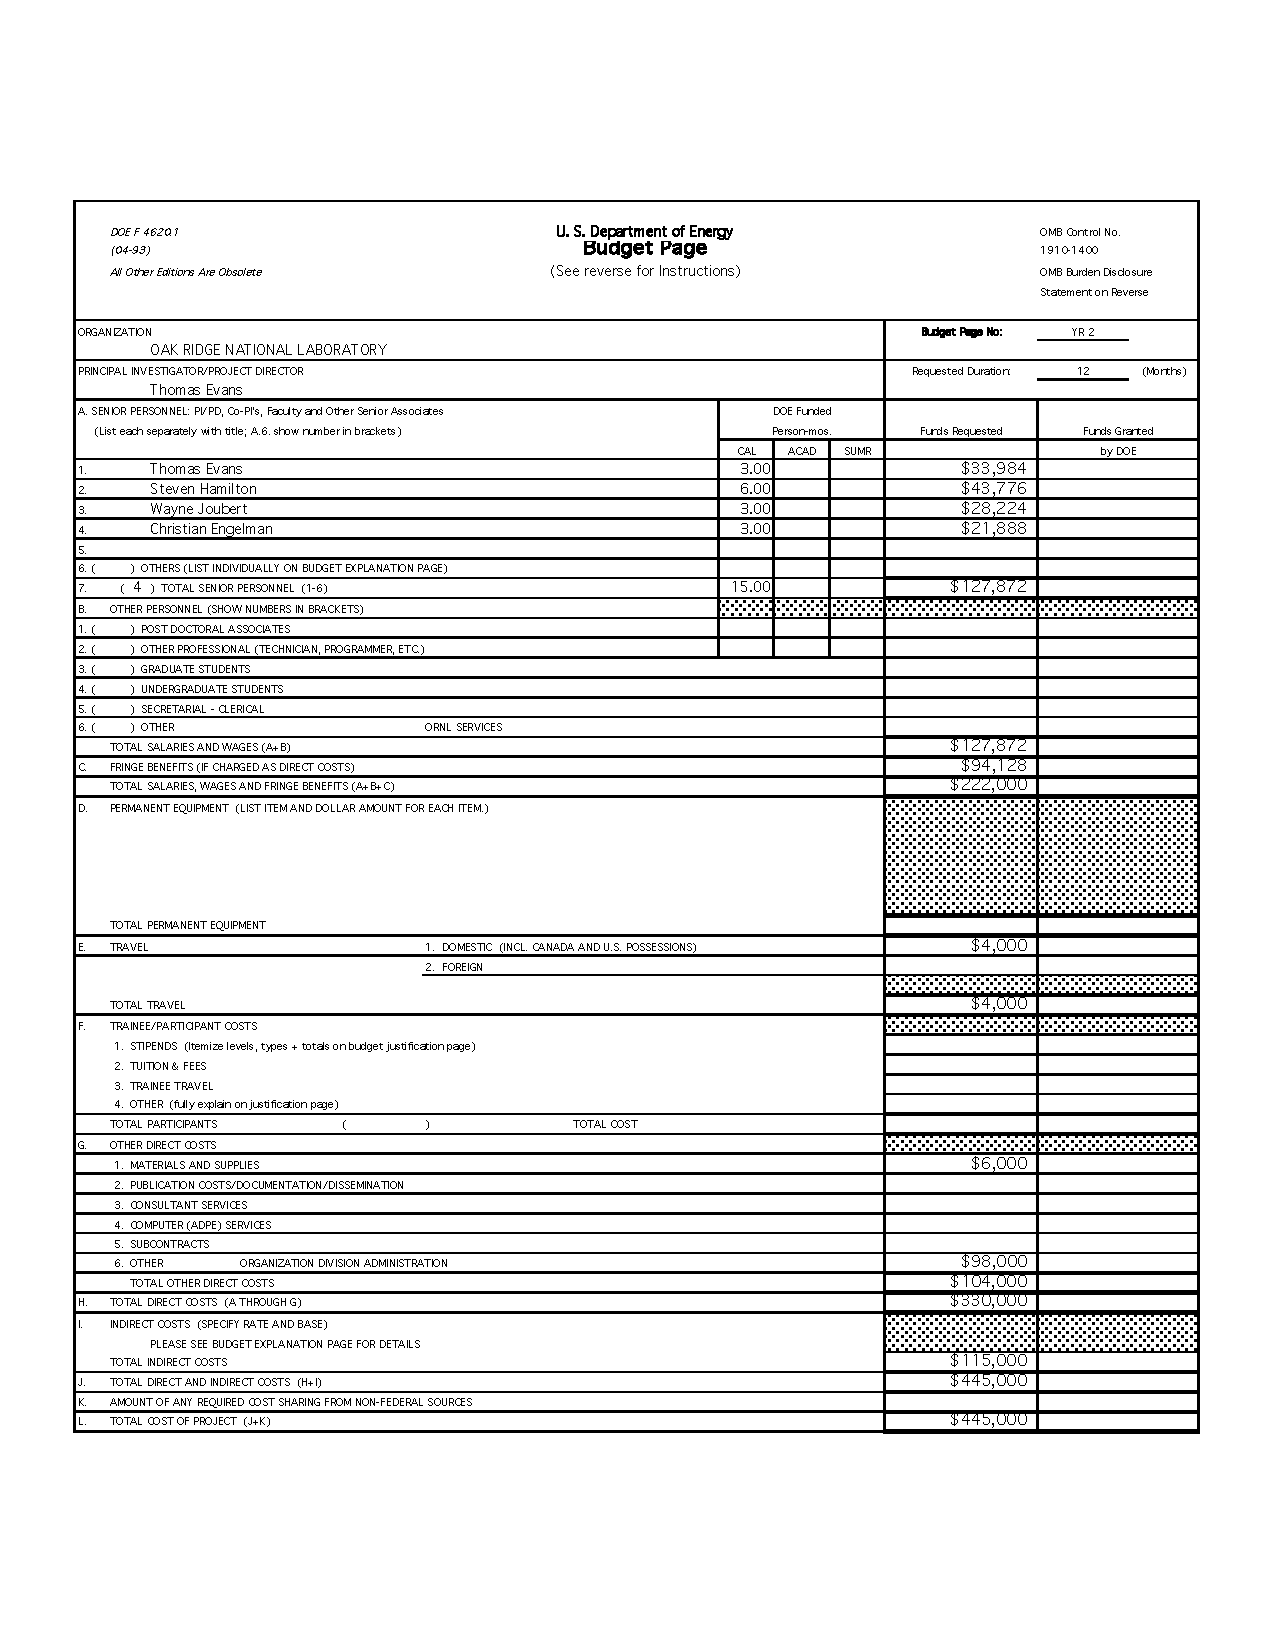
\includepdf[pages=-,pagecommand={\thispagestyle{fancy}},
noautoscale=true,scale=0.9] {supp/doe_4620_2}
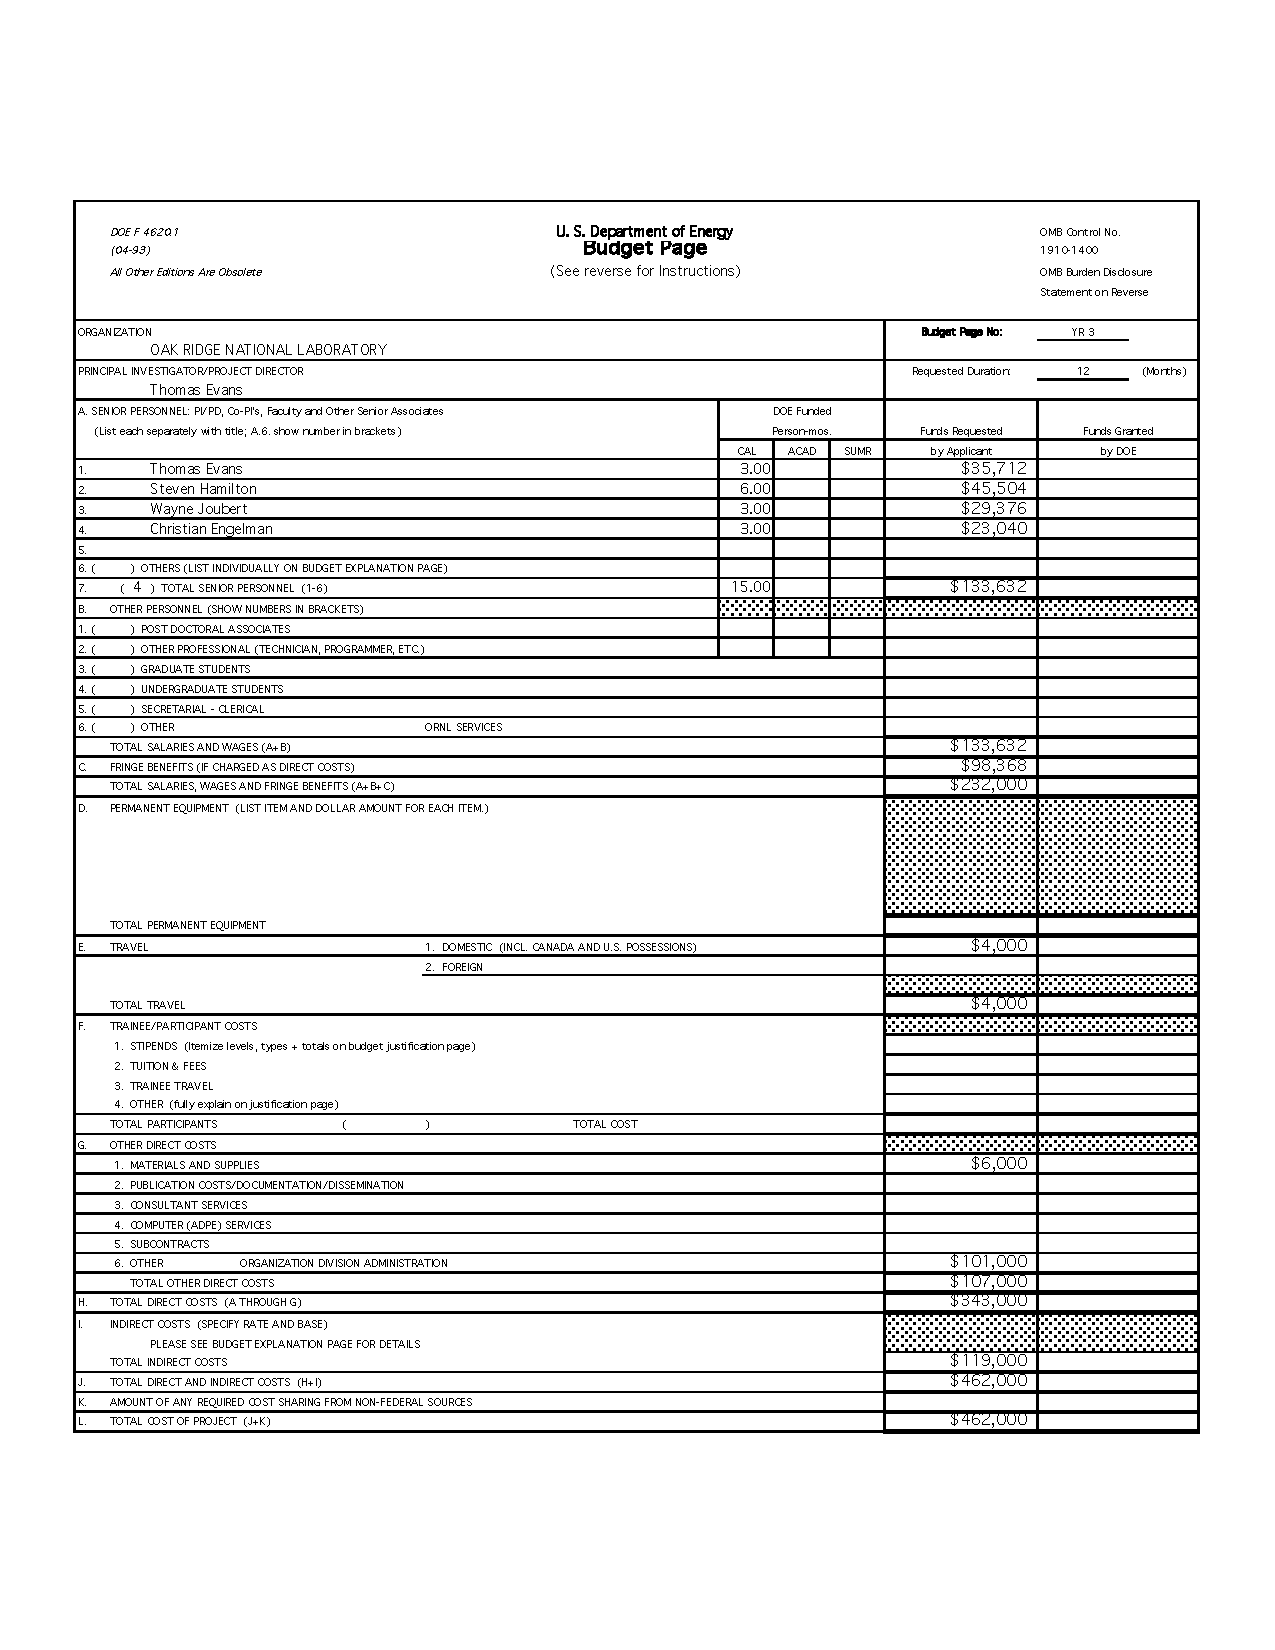
\includepdf[pages=-,pagecommand={\thispagestyle{fancy}},
noautoscale=true,scale=0.9] {supp/doe_4620_3}
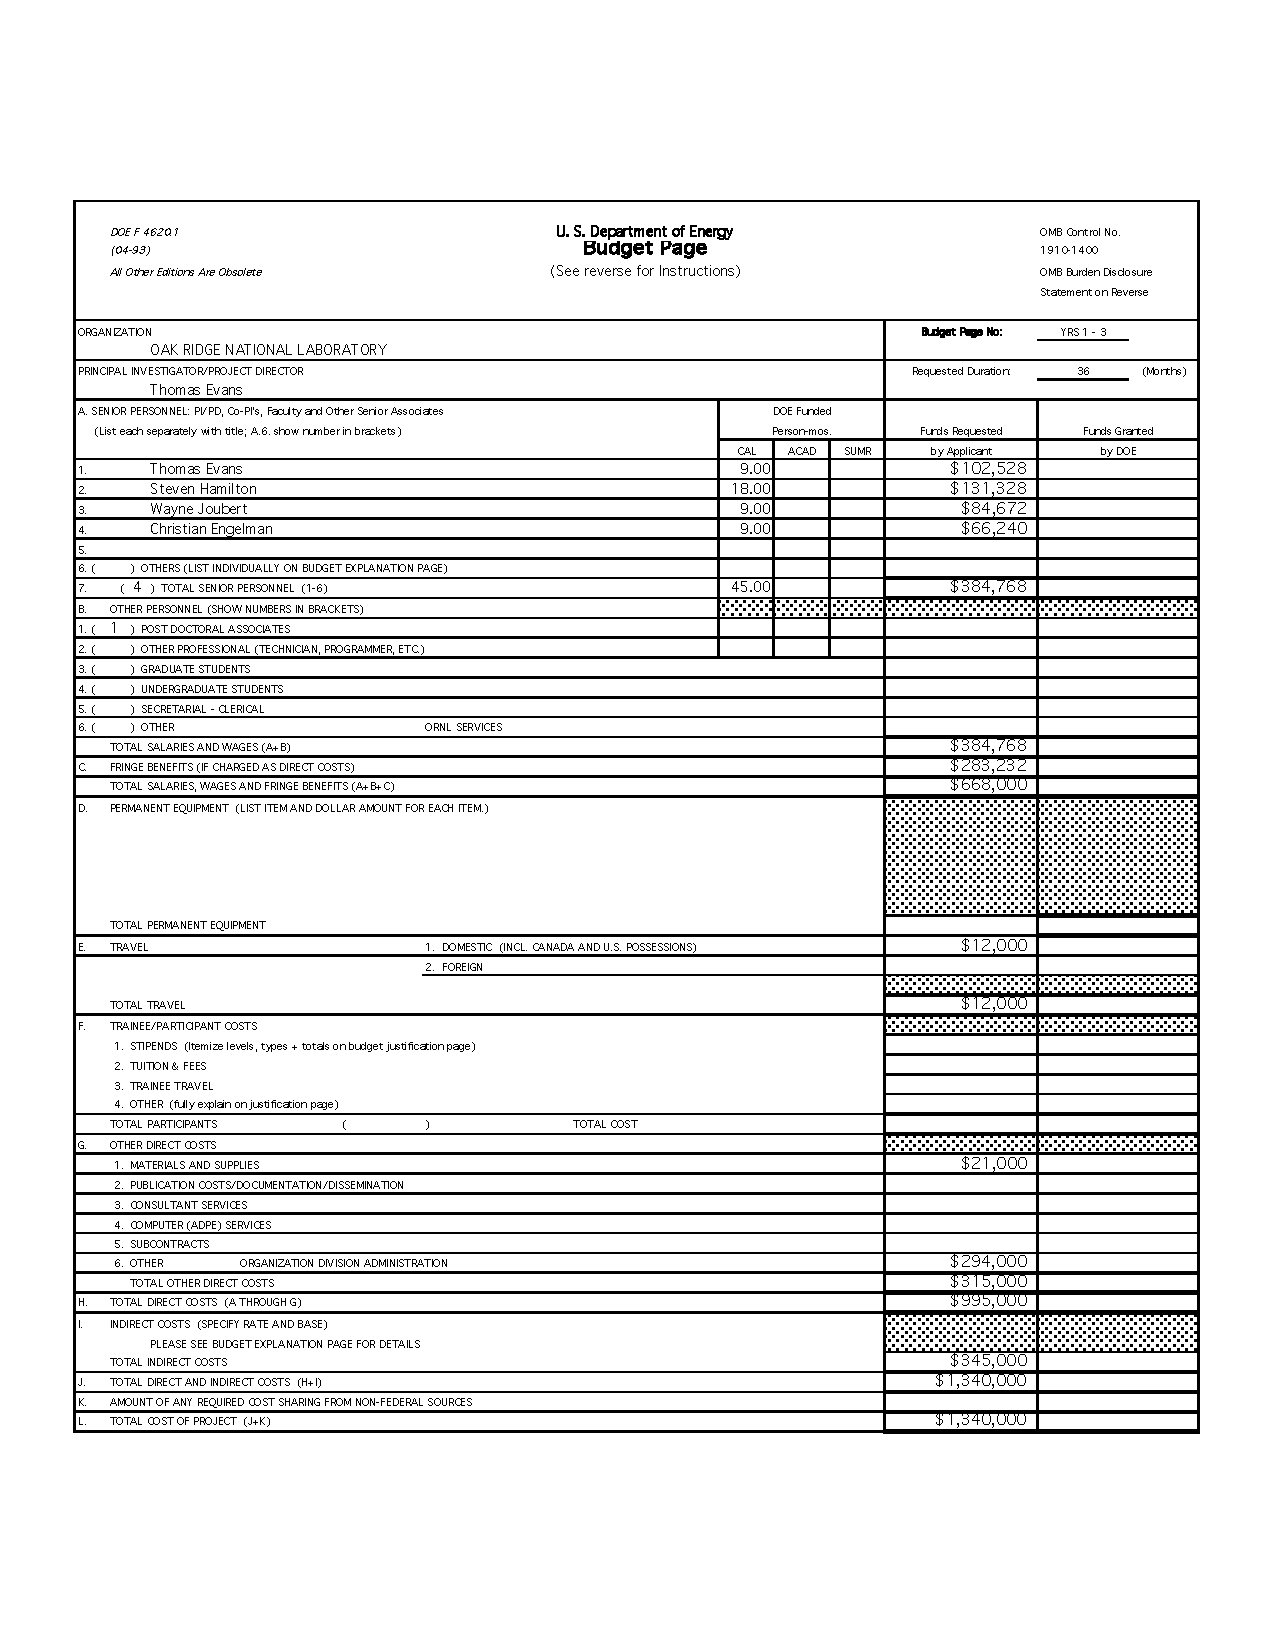
\includepdf[pages=-,pagecommand={\thispagestyle{fancy}},
noautoscale=true,scale=0.9] {supp/doe_4620_4}

\subsection*{ORNL Budget Explanation}
\addcontentsline{toc}{subsection}{\protect\numberline{}ORNL Budget Explanation}

Cost estimates presented in this proposal have been reclassified to be
comparable with proposals from other research institutions.  At the Oak Ridge
National Laboratory (ORNL), actual costs will be collected and reported in
accordance with the Department of Energy (DOE) approved cost accounting
system.  Total cost presented in this proposal and actual costs will be
equivalent as will the subtotal of direct and indirect costs.  Details of the
budget breakdown of all budget categories, including salaries, benefits and
fringe, and direct costs are described below.  In consideration of cost
estimates for ORNL staff support, it is important to understand that all ORNL
costs are covered by proposals such as this one.  There is no ``base'' funding
for DOE Office of Science multiprogram national laboratories, including ORNL.

\begin{description}

\item {\bf A. (1-6) Senior Personnel}
  %\vspace{2ex}
  
  The ORNL cost accounting system incorporates wage pools which are built
  around actual salaries for staff with similar salaries.  The salary figure
  listed for Senior Personnel represents the average salary for a staff
  scientist within a specific wage pool.  For budgeting purposes, one calendar
  month is assumed to be 150.0 hours.
  
  Support is requested for Drs. Christian Engelmann, Thomas Evans, Steven
  Hamilton and Wayne Joubert as detailed in the budget spreadsheets.
  Dr. Thomas Evans will serve as Research Coordinator and Project PI.

\item {\bf B. (1-6) Other Personnel}
  %\vspace{2ex}
  
  No funds are allocated toward other staff for this proposal.

\item {\bf C. Fringe Benefits}
  %\vspace{2ex}

  Fringe benefits are included in the ORNL employees wage pool rate and are
  estimated at 59.0\% for FY2012, decreasing to 48.0\% for FY2013--2017.

\item {\bf D. Permanent Equipment}
  %\vspace{2ex}
  
  No funds for permanent equipment are allocated.
 
\item {\bf E. Travel}
  %\vspace{2ex}
  
  Travel in the amount of \$4,000 per year is being included in the proposal
  in order to interact with M. Benzi and his students and present results at
  seminars.  This sum also allows travel to 1 to 2 meetings per year in order
  to present results of the project.

\item {\bf G. (1-6) Other Direct Costs}
  %\vspace{2ex}
  
  \begin{description}
    
  \item {\bf 1. Materials \& Supplies}
    %\vspace{2ex}
    
    Materials and supplies include general and miscellaneous supplies directly
    related to the project.  The additional budget for the first year is
    provided for software licenses for both toolkits needed to complete work
    for the proposal and collaboration software that will enable a virtual
    ``one-roof'' collaboration between ORNL and Emory.
    
  \item {\bf 6. Other --- Organization Burden Administration}
    %\vspace{2ex}
    
    Organizational Burden Administration costs include utilities (purchased
    utilities as well as laboratory staff associated with maintaining the
    utility systems), space charges (building maintenance), division
    managerial oversight, technical and administrative support, and other
    support personnel such as plant and equipment, instrumentation and
    controls, environmental, safety, and health, finance and budget, quality,
    and health physics provided for the general benefit of all staff and R\&D
    activities.  Inclusion of these costs is necessary to provide a full
    accounting of estimated cost for the project period.  All cost will be
    collected and reported in ORNL's cost accounting system, as approved by
    DOE.
  
  \end{description}

\end{description}

\pagebreak

%%---------------------------------------------------------------------------%%

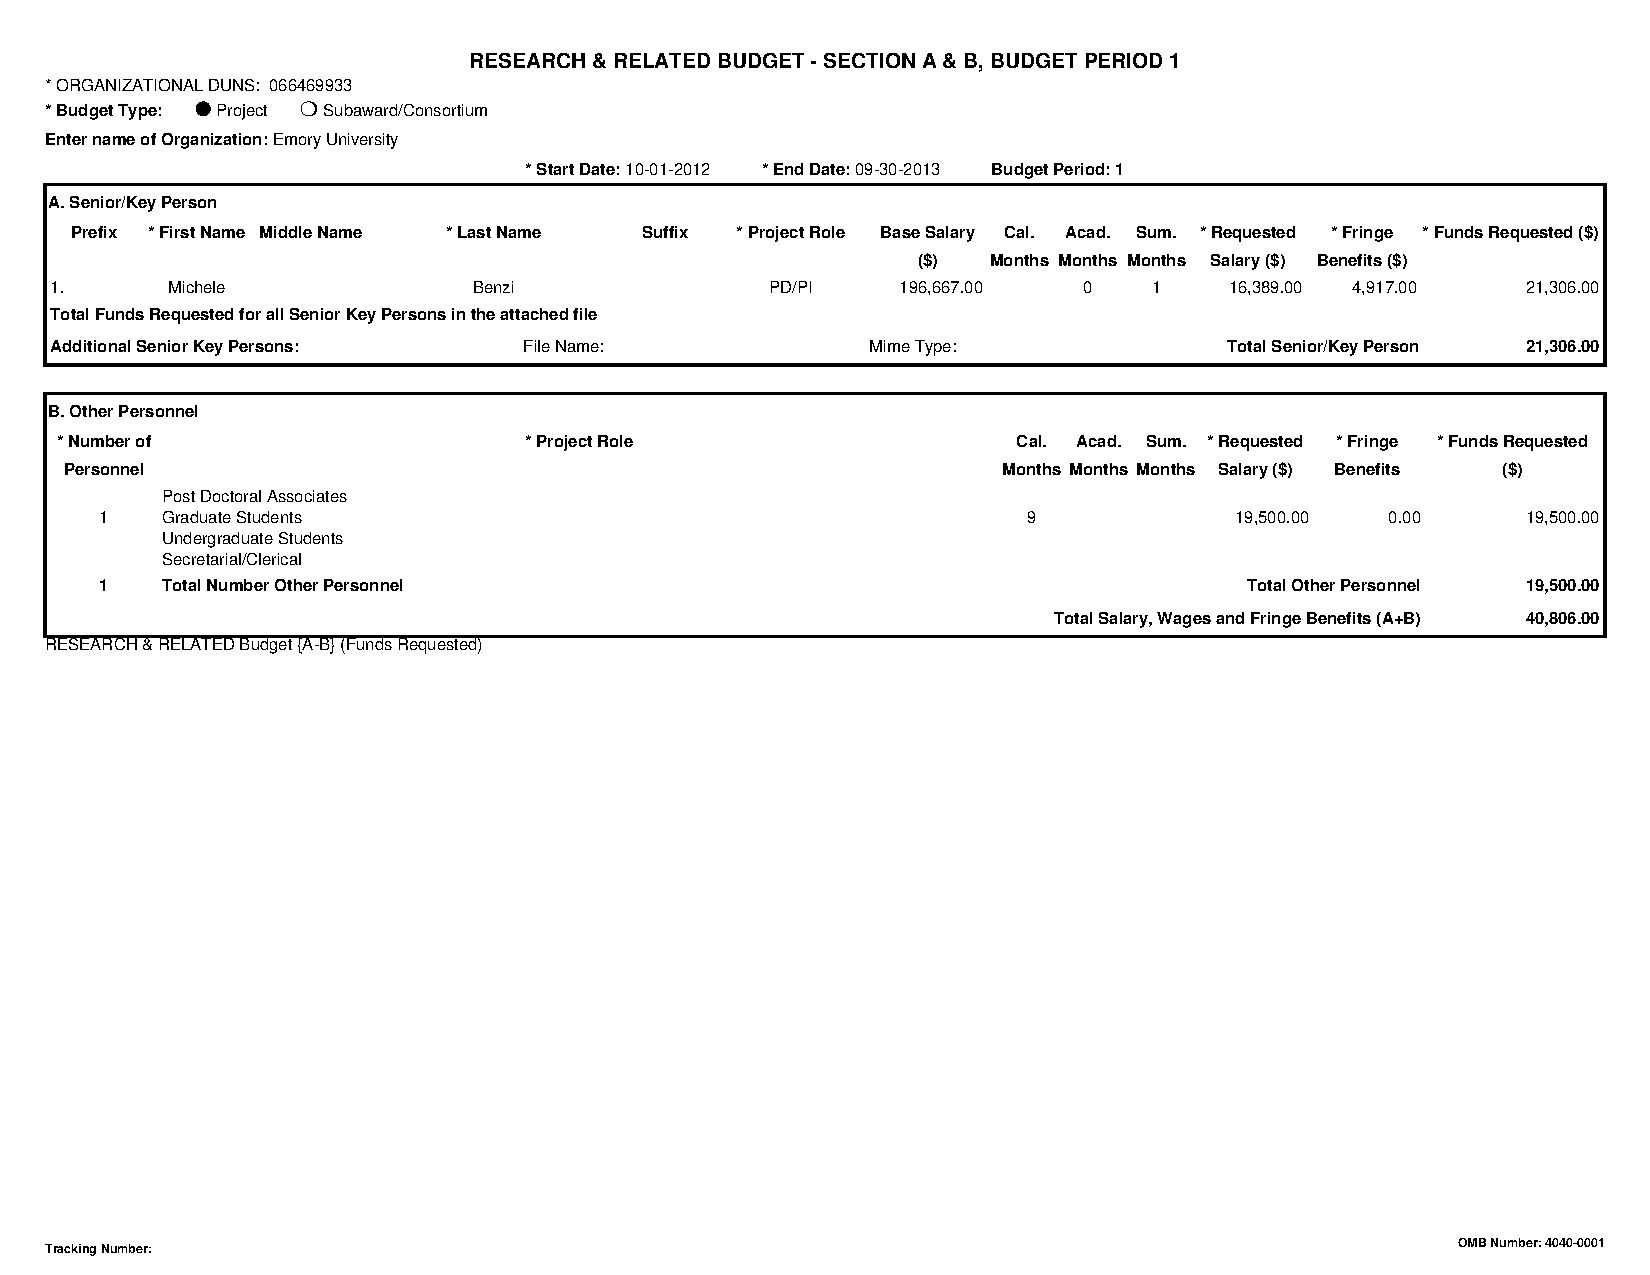
\includepdf[pages=1,pagecommand={\subsection*{Emory Budget}
  \thispagestyle{fancy}}, noautoscale=true,scale=0.7] {supp/emory_budget_pages}
\addcontentsline{toc}{subsection}{\protect\numberline{}Emory Budget}
\includepdf[pages=2-3,pagecommand={\thispagestyle{fancy}},
noautoscale=true,scale=0.7] {supp/emory_budget_pages}
\includepdf[pages=4,pagecommand={\thispagestyle{fancy}},
noautoscale=true,scale=0.7] {supp/emory_budget_pages}
\includepdf[pages=5-6,pagecommand={\thispagestyle{fancy}},
noautoscale=true,scale=0.7] {supp/emory_budget_pages}
\includepdf[pages=7,pagecommand={\thispagestyle{fancy}},
noautoscale=true,scale=0.7] {supp/emory_budget_pages}
\includepdf[pages=8-10,pagecommand={\thispagestyle{fancy}},
noautoscale=true,scale=0.7] {supp/emory_budget_pages}

\subsection*{Emory Budget Explanation}
\addcontentsline{toc}{subsection}{\protect\numberline{}Emory Budget
  Explanation}

\noindent {\bf Salary}

One month summer salary in each year of the project is requested to free the
PI from teaching in order to conduct a significant portion of the proposed
research. Fringe benefits for faculty members at Emory are currently 30\% of
salary. A 3\% raise per year is projected.

The proposed research provides an excellent opportunity for a motivated Ph.D.
student working on a dissertation in large-scale scientific computing on
emerging architectures.  The Ph.D. program in Computational Mathematics at
Emory University has a strong history of attracting top graduate students,
many of whom went on to successful careers in academia, government, and
industry, including several females.  Funds to support a full-time (academic
year) Ph.D.  student are requested for each of the three years of the project.
Student salary is \$19,500 for the first year, with a 3\% raise per year.
Additionally, funds to cover the student's enrollment fees totalling
\$2,813/year are being requested.

\medskip
\par\noindent 
{\bf Travel}

Travel support to attend meetings with the other project investigators plus
one relevant conference per year, for a total of \$6,116 in year one, \$6,353
year two, and \$6,598 in year three is requested.


\pagebreak
\endinput

%%---------------------------------------------------------------------------%%
%% end of budgets.tex
%%---------------------------------------------------------------------------%%

